\documentclass[a4paper,10pt]{article}
\usepackage[lmargin=2.0cm, rmargin=1.0cm,tmargin=3.5cm,bmargin=1.5cm]{geometry}
\usepackage{color,graphics}
\usepackage[export]{adjustbox}
\usepackage{lipsum}
\usepackage{multirow}
\usepackage{graphicx}
%\usepackage{lstlisting}

\usepackage{listings}
\usepackage[scaled=0.75]{helvet}

\begin{document}
\setcounter{secnumdepth}{-1} 

\begin{center}
\textbf{\LARGE Implement an application that stores big data in HBase using Hadoop.}
\end{center}

\raggedright Expt No: 8 \hfill \raggedleft May 27,2019 \\ 

\raggedright Author: Preethi V (186001005) \par 


\section{Aim}
To implement an application that stores big data in HBase using Hadoop.

\section{Description}
         	HBase is a distributed column-oriented database built on top of the Hadoop file system. It is an open-source project and is horizontally scalable. HBase is a data model that is similar to Google’s big table designed to provide quick random access to huge amounts of structured data. It leverages the fault tolerance provided by the Hadoop File System (HDFS).
			It is a part of the Hadoop ecosystem that provides random real-time read/write access to data in the Hadoop File System.One can store the data in HDFS either directly or through HBase. Data consumer reads/accesses the data in HDFS randomly using HBase. HBase sits on top of the Hadoop File System and provides read and write access.
	
\begin{figure}[h]
	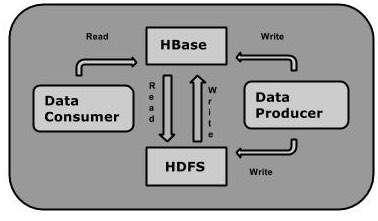
\includegraphics[scale=0.33,center]{0.jpg}
	\caption{Hadoop Random Access Databases.}
	\label{fig:1}
\end{figure}

\section{Procedure}

\begin{enumerate}
	\item Prepare a Virtual Machine Environment
	\item Install Java
	\item Install Hadoop
	\item Install HBase
\end{enumerate}	

\section{HBase Commands}
Write about HBase Commands
\begin{enumerate}
	\begin{itemize}
		\item Create:
			create a table in HBase with the specified name given according to the dictionary or specifications as per column family. In addition to this we can also pass some table-scope attributes 
			
			\begin{equation}
				 create <tablename>, <columnfamilyname>
			\end{equation}
		\item Put:			  
   		 It will put a celli'value' at defined or specified table or row or column.It will optionally coordinate time stamp.
			\begin{equation}
				put <'tablename'>,<'rowname'>,<'columnvalue'>,<'value'>
			\end{equation}
		\item Scan:
		    We can pass several optional specifications to this scan command to get more information about the tables present in the system.Scanner specifications may include one or more of the following attributes.These are TIMERANGE, FILTER, TIMESTAMP, LIMIT, MAXLENGTH, COLUMNS, CACHE, STARTROW and STOPROW.
			\begin{equation}
				scan <'tablename'>, {Optional parameters}
			\end{equation}

		\item Get:
		You will get a row or cell contents present in the table. In addition to that you can also add additional parameters to it like TIMESTAMP, TIMERANGE,VERSIONS, FILTERS, etc. to get a particular row or cell content. 
			\begin{equation}
				 get <'tablename'>, <'rowname'>, {< Additional parameters>}
			\end{equation}
		\item Disable:
			 This command will start disabling the named table.f table needs to be deleted or dropped, it has to disable first.
			\begin{equation}
				disable <tablename>
			\end{equation}
		This command will disable all the tables matching the given regex.The implementation is same as delete command (Except adding regex for matching).Once the table gets disable the user can able to delete the table from HBase.Before delete or dropping table, it should be disabled first.
		    \begin{equation}
				disable_all<"matching regex">
			\end{equation}
		\item Drop:
		    To delete the table present in HBase, first we have to disable it.    To drop the table present in HBase, first we have to disable it. So either table to drop or delete first the table should be disable using disable command.Here in above screenshot we are dropping table "education".Before execution of this command, it is necessary that you disable table "education".
		    \begin{equation}
				drop <table name>
			\end{equation}
	\end{itemize}
\end{enumerate}

\section{Output}

\begin{figure}[h]
	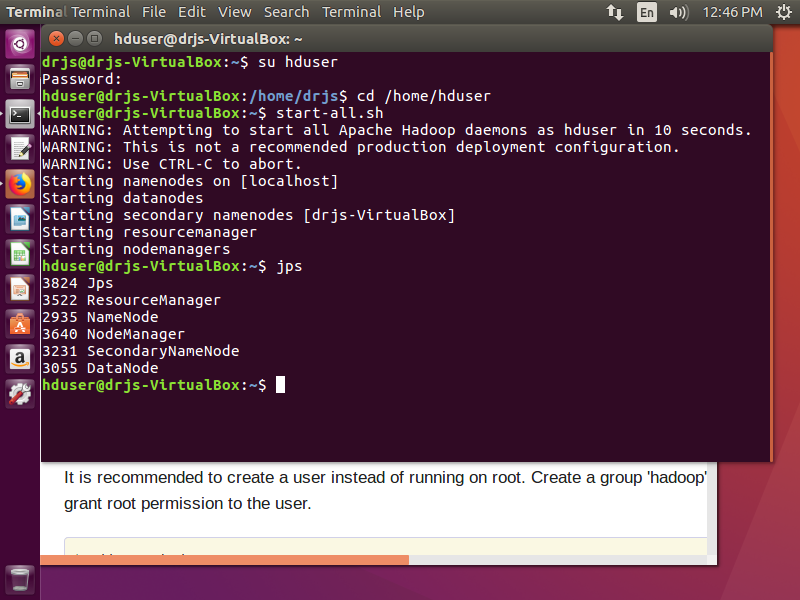
\includegraphics[scale=0.33,center]{1.png}
	\caption{Starting of Hadoop.}
	\label{fig:1}
\end{figure}

\begin{figure}[h]
	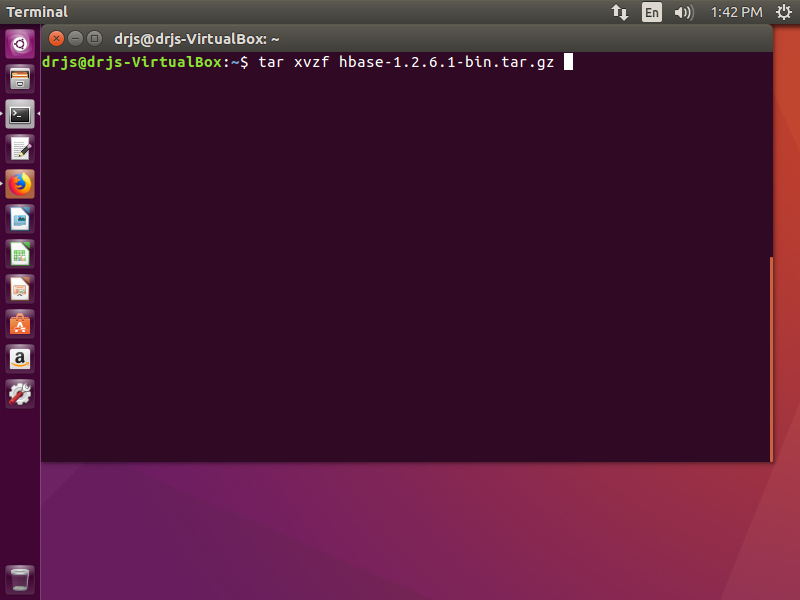
\includegraphics[scale=0.33,center]{2.png}
	\caption{Unzipping the hadoop file using tar command.}
	\label{fig:1}
\end{figure}	

\begin{figure}[h]
	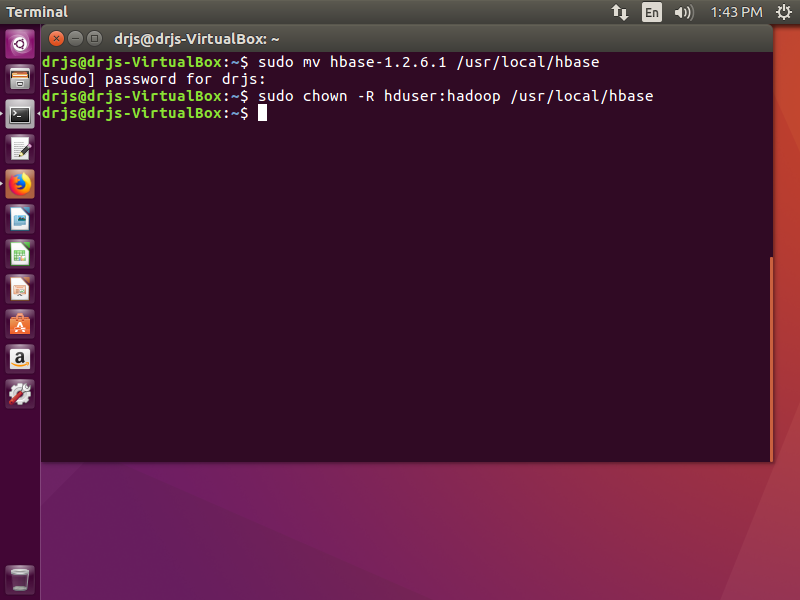
\includegraphics[scale=0.33,center]{3.png}
	\caption{Moving and changing the owner to /usr/local/hadoop.}
	\label{fig:1}
\end{figure}

\begin{figure}[h]
	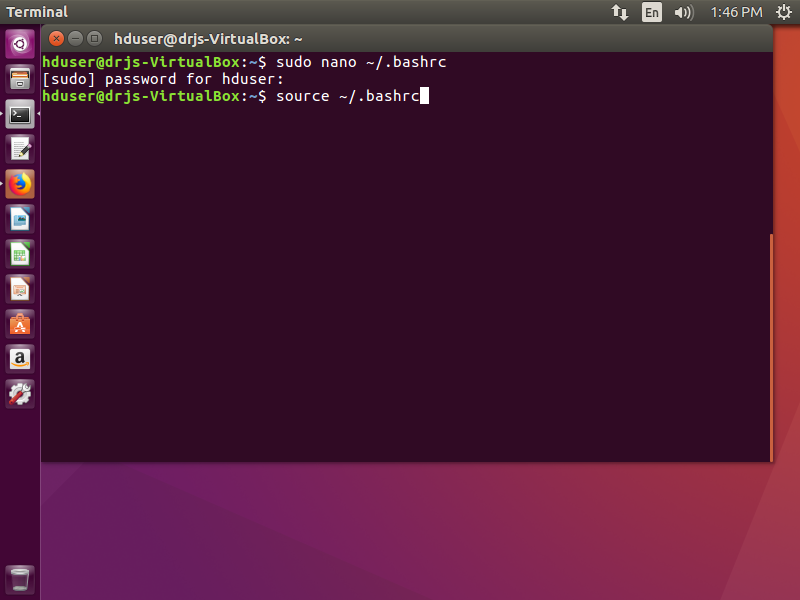
\includegraphics[scale=0.33,center]{4.png}
	\caption{Configuring bashrc.}
	\label{fig:1}
\end{figure}

\begin{figure}[h]
	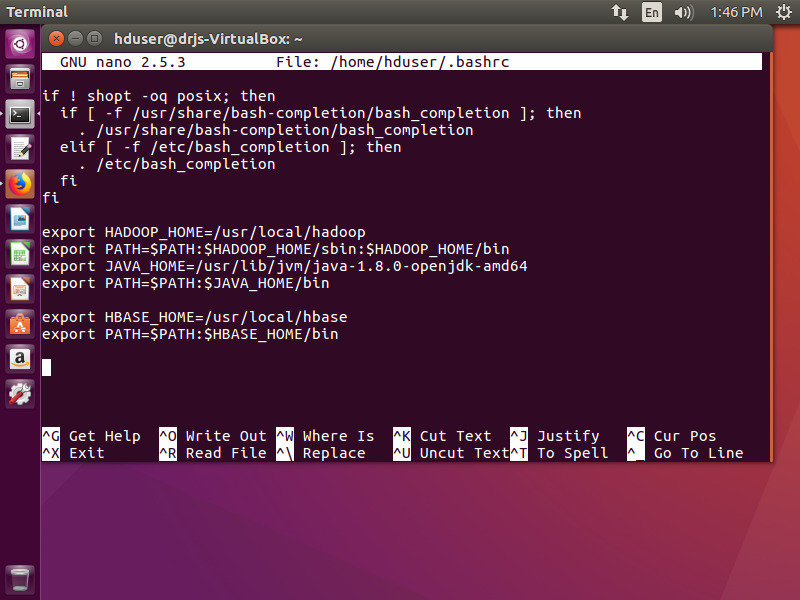
\includegraphics[scale=0.33,center]{5.png}
	\caption{Setting the hbase home and path.}
	\label{fig:1}
\end{figure}

\begin{figure}[h]
	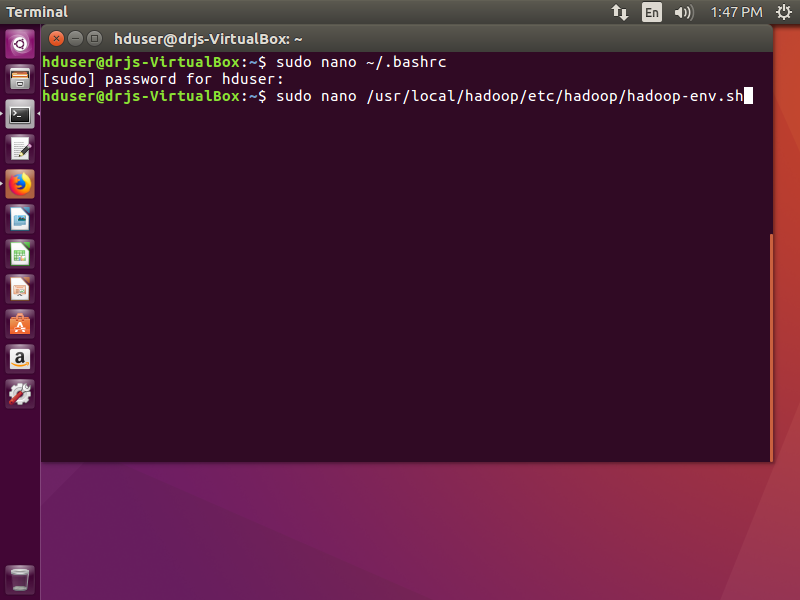
\includegraphics[scale=0.33,center]{6.png}
	\caption{Configuring hadoop-env.sh file.}
	\label{fig:1}
\end{figure}

\begin{figure}[h]
	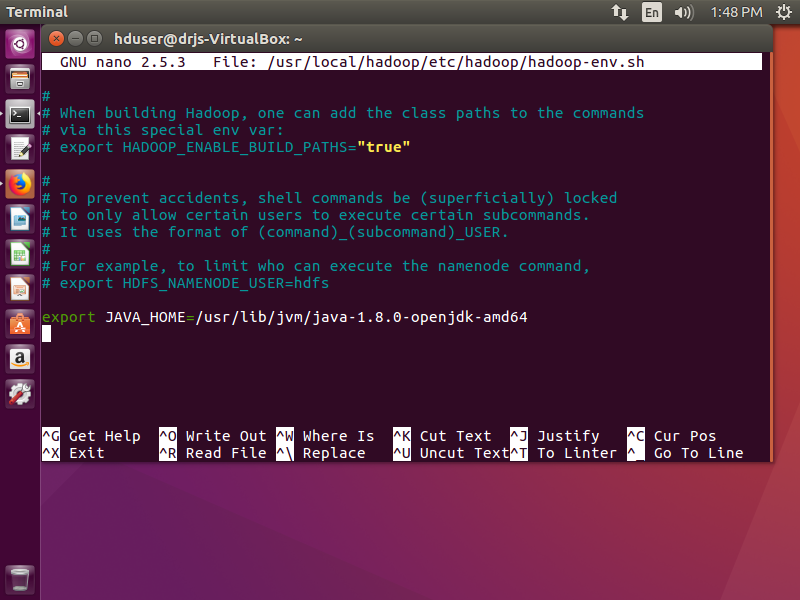
\includegraphics[scale=0.33,center]{7.png}
	\caption{Setting java path.}
	\label{fig:1}
\end{figure}

\begin{figure}[h]
	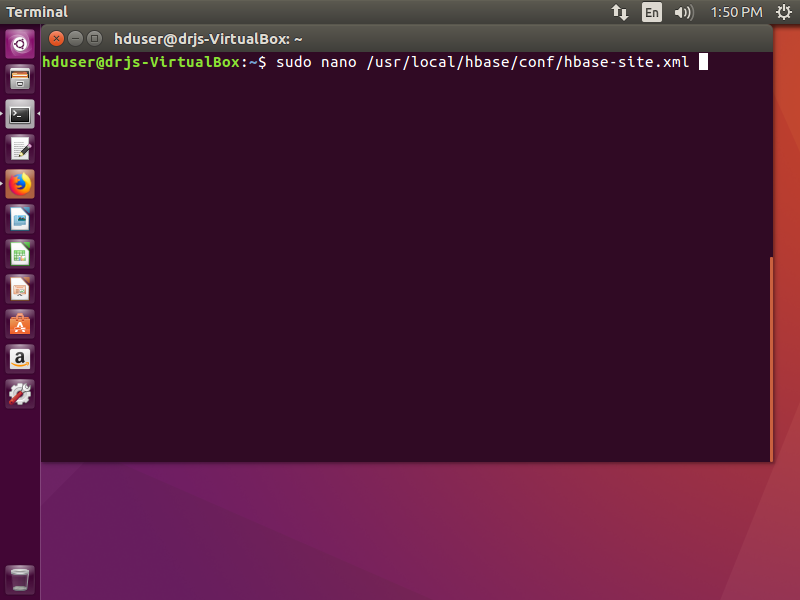
\includegraphics[scale=0.33,center]{8.png}
	\caption{Configuring hbase-site.xml file.}
	\label{fig:1}
\end{figure}

\begin{figure}[h]
	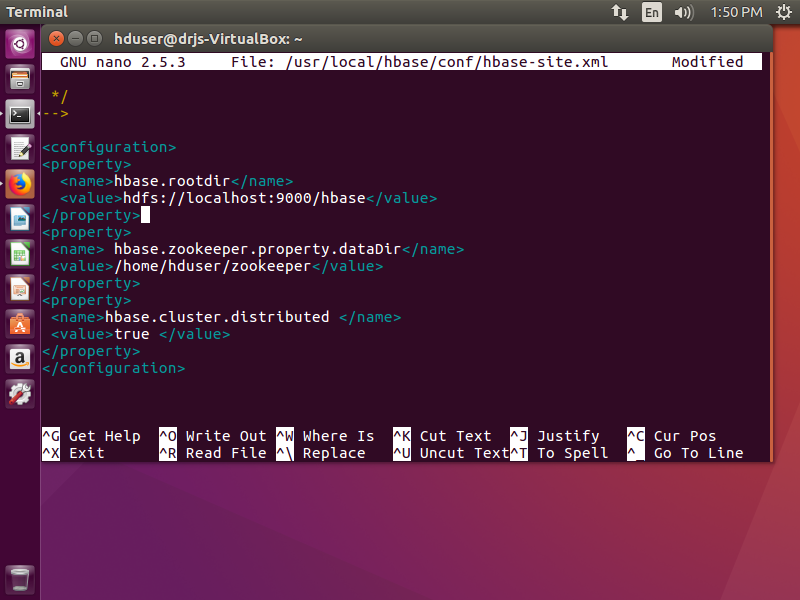
\includegraphics[scale=0.33,center]{9.png}
	\caption{hbase-site.xml.}
	\label{fig:1}
\end{figure}

\begin{figure}[h]
	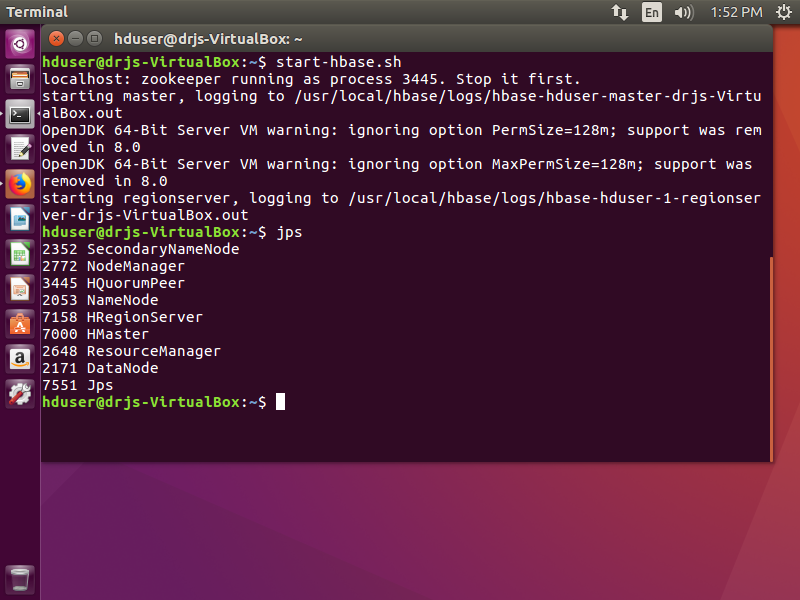
\includegraphics[scale=0.33,center]{10.png}
	\caption{Starting HBase.}
	\label{fig:1}
\end{figure}

\begin{figure}[h]
	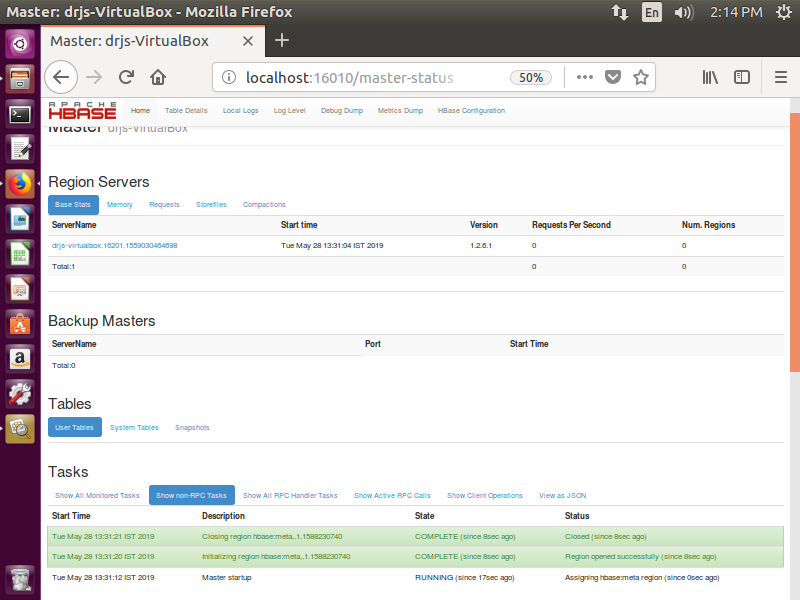
\includegraphics[scale=0.33,center]{19.png}
	\caption{Master status.}
	\label{fig:1}
\end{figure}

\begin{figure}[h]
	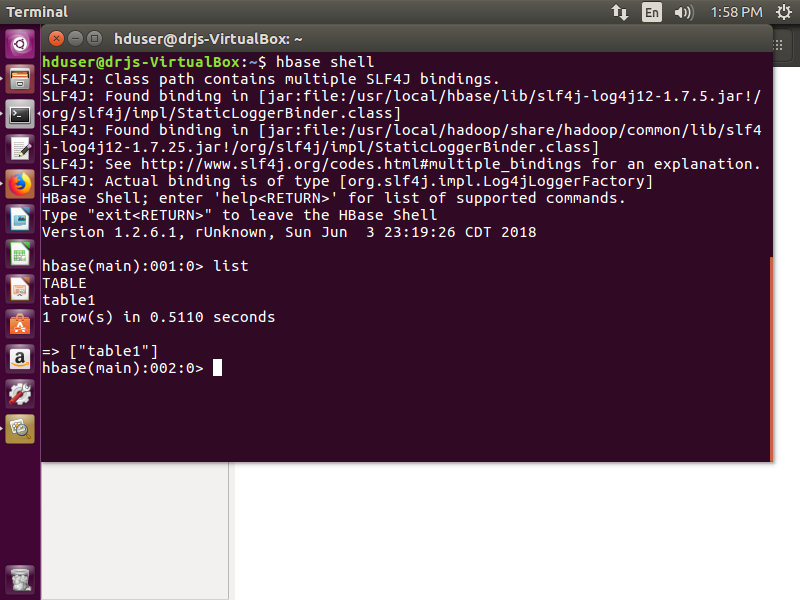
\includegraphics[scale=0.33,center]{11.png}
	\caption{hbase shell.}
	\label{fig:1}
\end{figure}

\begin{figure}[h]
	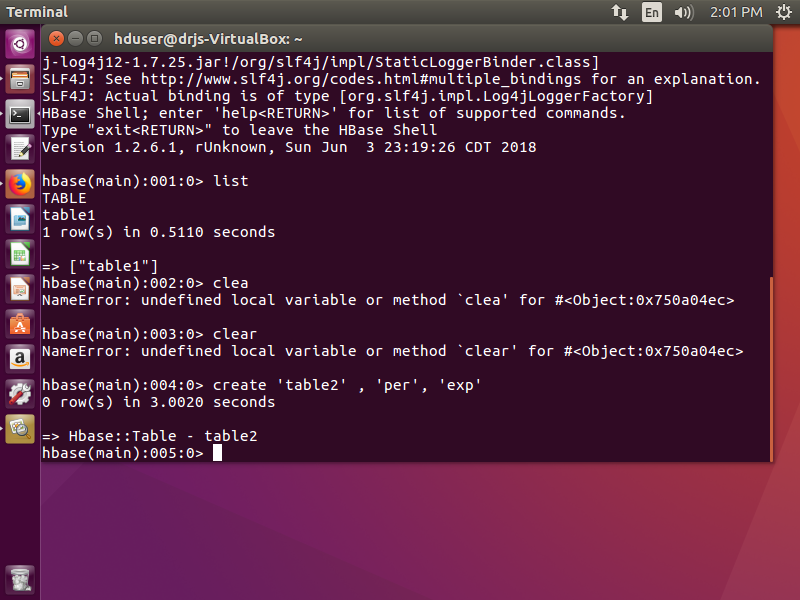
\includegraphics[scale=0.33,center]{12.png}
	\caption{Creation of table.}
	\label{fig:1}
\end{figure}

\begin{figure}[h]
	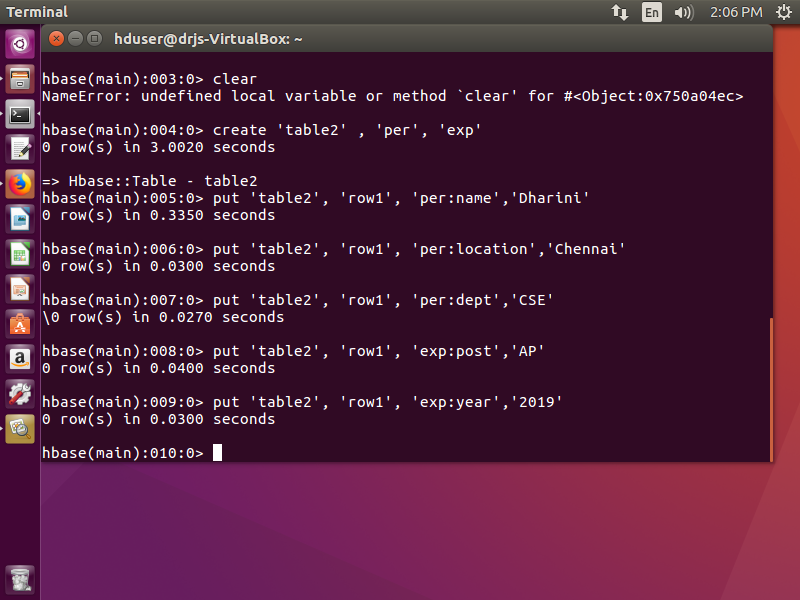
\includegraphics[scale=0.33,center]{13.png}
	\caption{Inserting rows using "put".}
	\label{fig:1}
\end{figure}

\begin{figure}[h]
	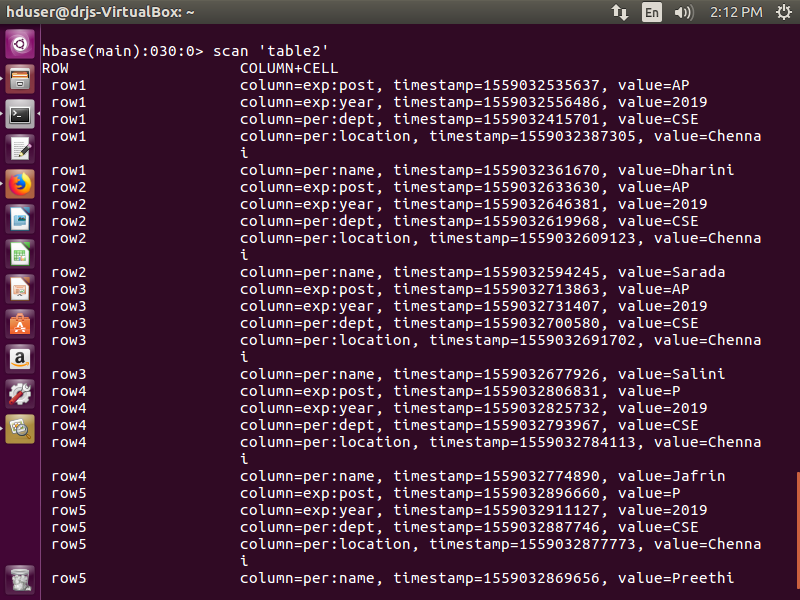
\includegraphics[scale=0.33,center]{17.png}
	\caption{Displaying the rows in table using "scan".}
	\label{fig:1}
\end{figure}

\begin{figure}[h]
	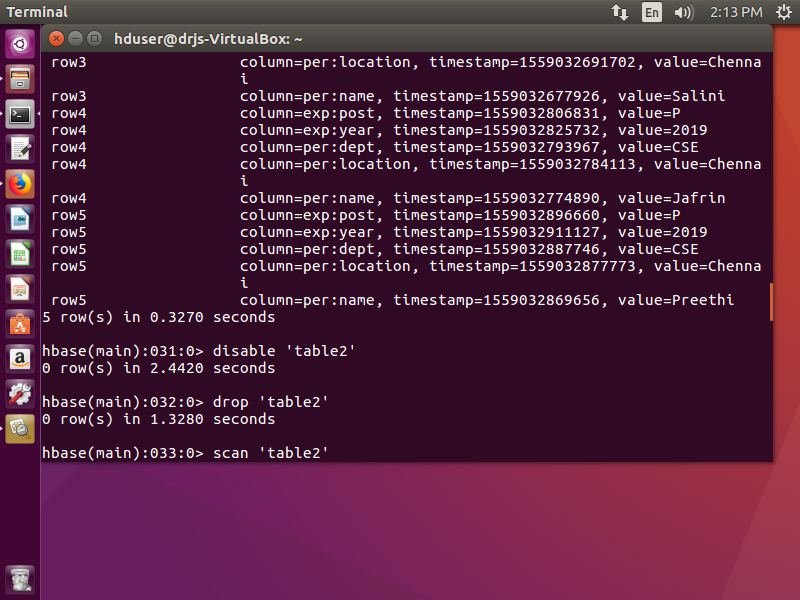
\includegraphics[scale=0.33,center]{18.png}
	\caption{Disabling and Dropping the table 2.}
	\label{fig:1}
\end{figure}

\end{figure}


\end{document}
